% Source: tex/chapters/ch05/10_新興技術のテストと新興技術によるテスト.tex
\subsection{新興技術のテストと新興技術によるテスト}
新興技術は、テスト対象として新しい課題を生む一方で、テスト活動を支援する手段にもなる。この章では、「新興技術をテストする」と「新興技術を使ってテストする」を分けて理解する。

\begin{figure}[htbp]
\centering
\IfFileExists{assets/fig-ch05-14.png}{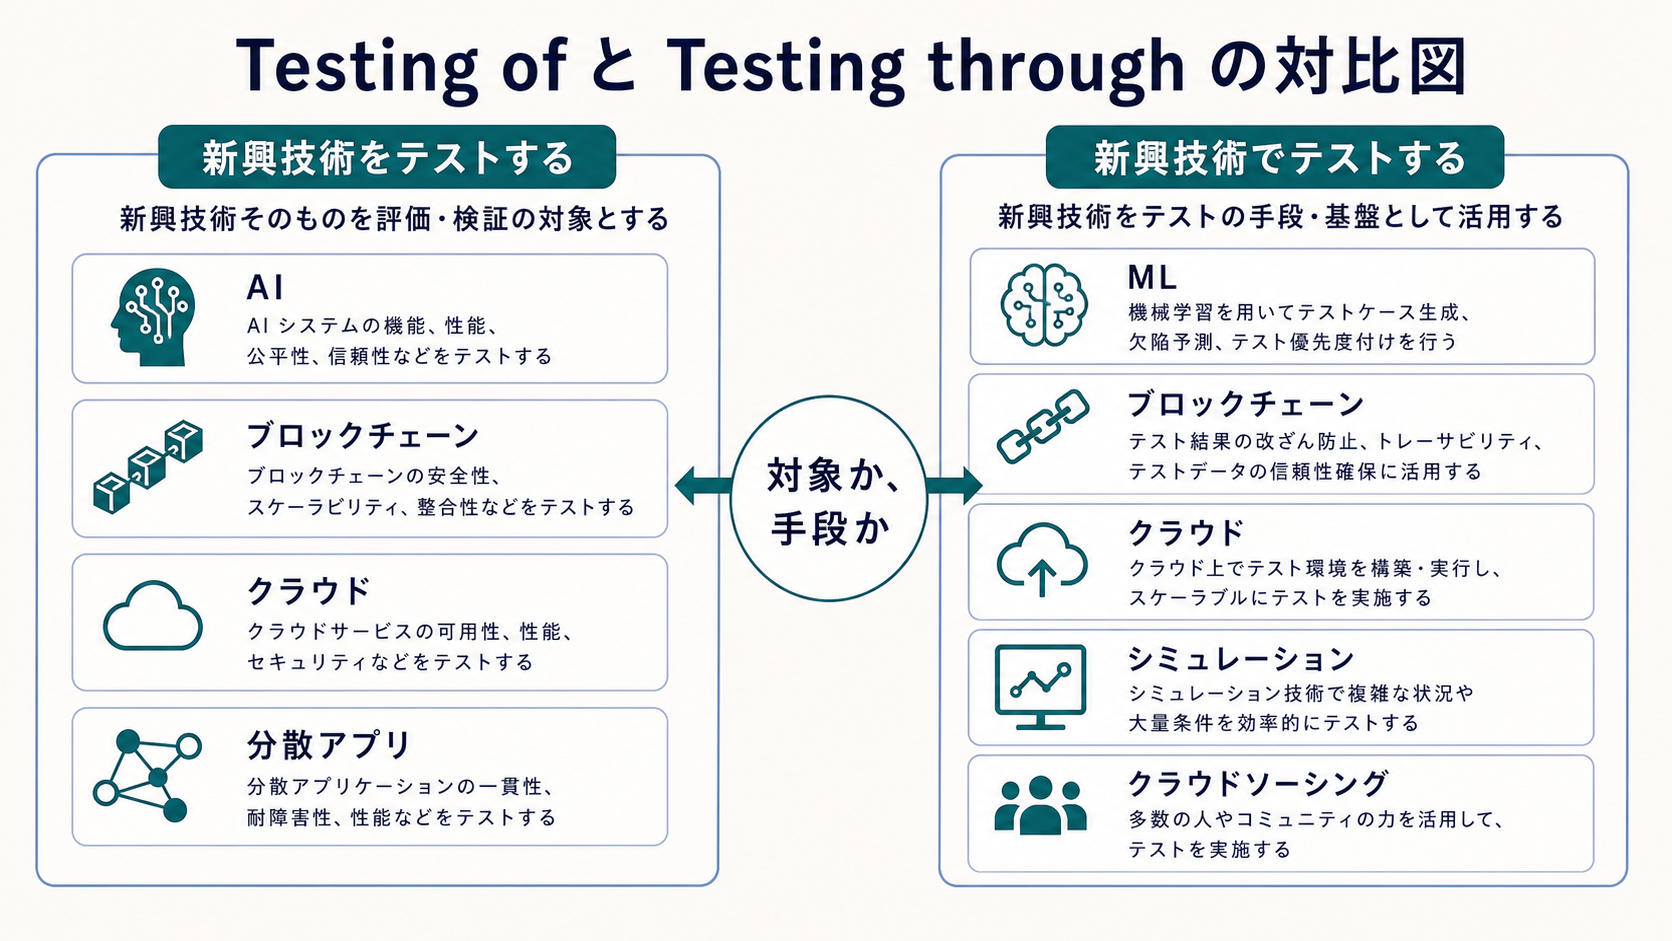
\includegraphics[width=0.96\linewidth]{assets/fig-ch05-14.png}}{\fbox{\parbox[c][48mm][c]{0.9\linewidth}{\centering 画像生成待ち\\Testing of と Testing through の対比図}}}
\caption{Testing of と Testing through の対比図}
\label{fig:ch05-14}
\end{figure}
